%!TEX TS-program = xelatex
\documentclass[10pt,oneside]{article}
\usepackage[fontsize=9pt]{scrextend}

\usepackage[english]{babel}

\usepackage{amsmath,amssymb,amsfonts}
\usepackage[utf8]{inputenc}
\usepackage[T1]{fontenc}
\usepackage{stix2}
\usepackage[scaled]{helvet}
\usepackage[scaled]{inconsolata}

\usepackage{lastpage}

\usepackage{setspace}

\usepackage{ccicons}

\usepackage[hang,flushmargin]{footmisc}

\usepackage{geometry}

\setlength{\parindent}{0pt}
\setlength{\parskip}{6pt plus 2pt minus 1pt}

\usepackage{fancyhdr}
\renewcommand{\headrulewidth}{0pt}\providecommand{\tightlist}{%
  \setlength{\itemsep}{0pt}\setlength{\parskip}{0pt}}

\makeatletter
\newcounter{tableno}
\newenvironment{tablenos:no-prefix-table-caption}{
  \caption@ifcompatibility{}{
    \let\oldthetable\thetable
    \let\oldtheHtable\theHtable
    \renewcommand{\thetable}{tableno:\thetableno}
    \renewcommand{\theHtable}{tableno:\thetableno}
    \stepcounter{tableno}
    \captionsetup{labelformat=empty}
  }
}{
  \caption@ifcompatibility{}{
    \captionsetup{labelformat=default}
    \let\thetable\oldthetable
    \let\theHtable\oldtheHtable
    \addtocounter{table}{-1}
  }
}
\makeatother

\usepackage{array}
\newcommand{\PreserveBackslash}[1]{\let\temp=\\#1\let\\=\temp}
\let\PBS=\PreserveBackslash

\usepackage[breaklinks=true]{hyperref}
\hypersetup{colorlinks,%
citecolor=blue,%
filecolor=blue,%
linkcolor=blue,%
urlcolor=blue}
\usepackage{url}

\usepackage{caption}
\setcounter{secnumdepth}{0}
\usepackage{cleveref}

\usepackage{graphicx}
\makeatletter
\def\maxwidth{\ifdim\Gin@nat@width>\linewidth\linewidth
\else\Gin@nat@width\fi}
\makeatother
\let\Oldincludegraphics\includegraphics
\renewcommand{\includegraphics}[1]{\Oldincludegraphics[width=\maxwidth]{#1}}

\usepackage{longtable}
\usepackage{booktabs}

\usepackage{color}
\usepackage{fancyvrb}
\newcommand{\VerbBar}{|}
\newcommand{\VERB}{\Verb[commandchars=\\\{\}]}
\DefineVerbatimEnvironment{Highlighting}{Verbatim}{commandchars=\\\{\}}
% Add ',fontsize=\small' for more characters per line
\usepackage{framed}
\definecolor{shadecolor}{RGB}{248,248,248}
\newenvironment{Shaded}{\begin{snugshade}}{\end{snugshade}}
\newcommand{\KeywordTok}[1]{\textcolor[rgb]{0.13,0.29,0.53}{\textbf{#1}}}
\newcommand{\DataTypeTok}[1]{\textcolor[rgb]{0.13,0.29,0.53}{#1}}
\newcommand{\DecValTok}[1]{\textcolor[rgb]{0.00,0.00,0.81}{#1}}
\newcommand{\BaseNTok}[1]{\textcolor[rgb]{0.00,0.00,0.81}{#1}}
\newcommand{\FloatTok}[1]{\textcolor[rgb]{0.00,0.00,0.81}{#1}}
\newcommand{\ConstantTok}[1]{\textcolor[rgb]{0.00,0.00,0.00}{#1}}
\newcommand{\CharTok}[1]{\textcolor[rgb]{0.31,0.60,0.02}{#1}}
\newcommand{\SpecialCharTok}[1]{\textcolor[rgb]{0.00,0.00,0.00}{#1}}
\newcommand{\StringTok}[1]{\textcolor[rgb]{0.31,0.60,0.02}{#1}}
\newcommand{\VerbatimStringTok}[1]{\textcolor[rgb]{0.31,0.60,0.02}{#1}}
\newcommand{\SpecialStringTok}[1]{\textcolor[rgb]{0.31,0.60,0.02}{#1}}
\newcommand{\ImportTok}[1]{#1}
\newcommand{\CommentTok}[1]{\textcolor[rgb]{0.56,0.35,0.01}{\textit{#1}}}
\newcommand{\DocumentationTok}[1]{\textcolor[rgb]{0.56,0.35,0.01}{\textbf{\textit{#1}}}}
\newcommand{\AnnotationTok}[1]{\textcolor[rgb]{0.56,0.35,0.01}{\textbf{\textit{#1}}}}
\newcommand{\CommentVarTok}[1]{\textcolor[rgb]{0.56,0.35,0.01}{\textbf{\textit{#1}}}}
\newcommand{\OtherTok}[1]{\textcolor[rgb]{0.56,0.35,0.01}{#1}}
\newcommand{\FunctionTok}[1]{\textcolor[rgb]{0.00,0.00,0.00}{#1}}
\newcommand{\VariableTok}[1]{\textcolor[rgb]{0.00,0.00,0.00}{#1}}
\newcommand{\ControlFlowTok}[1]{\textcolor[rgb]{0.13,0.29,0.53}{\textbf{#1}}}
\newcommand{\OperatorTok}[1]{\textcolor[rgb]{0.81,0.36,0.00}{\textbf{#1}}}
\newcommand{\BuiltInTok}[1]{#1}
\newcommand{\ExtensionTok}[1]{#1}
\newcommand{\PreprocessorTok}[1]{\textcolor[rgb]{0.56,0.35,0.01}{\textit{#1}}}
\newcommand{\AttributeTok}[1]{\textcolor[rgb]{0.77,0.63,0.00}{#1}}
\newcommand{\RegionMarkerTok}[1]{#1}
\newcommand{\InformationTok}[1]{\textcolor[rgb]{0.56,0.35,0.01}{\textbf{\textit{#1}}}}
\newcommand{\WarningTok}[1]{\textcolor[rgb]{0.56,0.35,0.01}{\textbf{\textit{#1}}}}
\newcommand{\AlertTok}[1]{\textcolor[rgb]{0.94,0.16,0.16}{#1}}
\newcommand{\ErrorTok}[1]{\textcolor[rgb]{0.64,0.00,0.00}{\textbf{#1}}}
\newcommand{\NormalTok}[1]{#1}

\newlength{\cslhangindent}
\setlength{\cslhangindent}{1.5em}
\newlength{\csllabelwidth}
\setlength{\csllabelwidth}{3em}
\newenvironment{CSLReferences}[3] % #1 hanging-ident, #2 entry spacing
 {% don't indent paragraphs
  \setlength{\parindent}{0pt}
  % turn on hanging indent if param 1 is 1
  \ifodd #1 \everypar{\setlength{\hangindent}{\cslhangindent}}\ignorespaces\fi
  % set entry spacing
  \ifnum #2 > 0
  \setlength{\parskip}{#2\baselineskip}
  \fi
 }%
 {}
\usepackage{calc} % for \widthof, \maxof
\newcommand{\CSLBlock}[1]{#1\hfill\break}
\newcommand{\CSLLeftMargin}[1]{\parbox[t]{\maxof{\widthof{#1}}{\csllabelwidth}}{#1}}
\newcommand{\CSLRightInline}[1]{\parbox[t]{\linewidth}{#1}}
\newcommand{\CSLIndent}[1]{\hspace{\cslhangindent}#1}\usepackage[table,dvipsnames]{xcolor}

\geometry{includemp,
            letterpaper,
            top=2.4cm,
            bottom=2.4cm,
            left=1.0cm,
            right=1.0cm,
            marginparwidth=5cm,
            marginparsep=1.0cm}

\usepackage[singlelinecheck=off]{caption}

\captionsetup{
  font={small},
  labelfont={bf},
  format=plain,
  labelsep=quad
}

\usepackage{floatrow}

\floatsetup[figure]{margins=hangright,
              facing=no,
              capposition=beside,
              capbesideposition={center,outside},
              floatwidth=\textwidth}

% \floatsetup[table]{margins=hangright,
%              facing=no,
%              capposition=beside,
%              capbesideposition={center,outside},
%              floatwidth=\textwidth}

\pagestyle{plain}

\setcounter{secnumdepth}{5}

\usepackage{titlesec}

\titleformat{\section}[block]
{\normalfont\large\sffamily}
{\thesection}{.5em}{\titlerule\\[.8ex]\bfseries}

\titleformat{\subsection}[runin]
{\normalfont\fontseries{b}\selectfont\filright\sffamily}
{\thesubsection.}{.5em}{}

\titleformat{\subsubsection}[runin]
{\normalfont\itshape\rmfamily\bfseries}{\thesubsubsection}{1em}{}

\fancypagestyle{firstpage}
{
   \fancyhf{}
   \renewcommand{\headrulewidth}{0pt}
   \fancyfoot[R]{\footnotesize\ccby}
   \fancyfoot[L]{\footnotesize\sffamily\today}
}

\fancypagestyle{normal}
{
  \fancyhf{}
  \fancyfoot[R]{\footnotesize\sffamily\thepage\ of \pageref*{LastPage}}
}

\usepackage{tikz}
\begin{document}
\pagestyle{normal}
\thispagestyle{firstpage}

\newcommand{\colorRule}[3][black]{\textcolor[HTML]{#1}{\rule{#2}{#3}}}

\noindent {\LARGE \textbf{\textsf{Template to prepare preprints and
manuscripts using markdown and github actions}}}

\medskip
\begin{flushleft}
{\small
%
\href{https://orcid.org/0000-0002-6506-6487}{Michael D.\,Catchen}%
%
\,\textsuperscript{1,2}
\vskip 1em
\textsuperscript{1}\,McGill University; \textsuperscript{2}\,Québec
Centre for Biodiversity Sciences\\
\vskip 1em
\textbf{Correspondance to:}\\
Michael D. Catchen --- \texttt{michael.catchen@mail.mcgill.ca}\\
}
\end{flushleft}

\vskip 2em
\makebox[0pt][l]{\colorRule[CCCCCC]{2.0\textwidth}{0.5pt}}
\vskip 2em
\noindent

\marginpar{\vskip 1em\flushright
{\small{\bfseries Keywords}:\par
pandoc\\pandoc-crossref\\github actions\\}
}




        {\bfseries Purpose:}\,This template provides a series of scripts
to render a markdown document into an interactive website and a series
of PDFs.\\%
        {\bfseries Motivation:}\,It makes collaborating on text with
GitHub easier, and means that we never need to think about the
output.\\%
        {\bfseries Internals:}\,GitHub actions and a series of python
scritpts. The markdown is handled with \texttt{pandoc}.\\%
    

\vskip 2em
\makebox[0pt][l]{\colorRule[CCCCCC]{2.0\textwidth}{0.5pt}}
\vskip 2em

Forecasting in ecology. Forecasting in weather, introduce computers.

Future is uncertain, how do we best act given a forecast?

We have some goal state for the future, and some estimate of what the
state of the world will be given a set of actions.

Brief summary of decision theory.

Transition to theme of optimization given unknown information. In face
of uncertainty, decision making is an optimization problem. Frame
optimization problem mathematically an introduce concept of
solution-space and constraint.

Transition to how this is applied in ecology. Introduce idea of
monitoring network. Transition to specifics of this thesis.

\begin{figure}
\centering
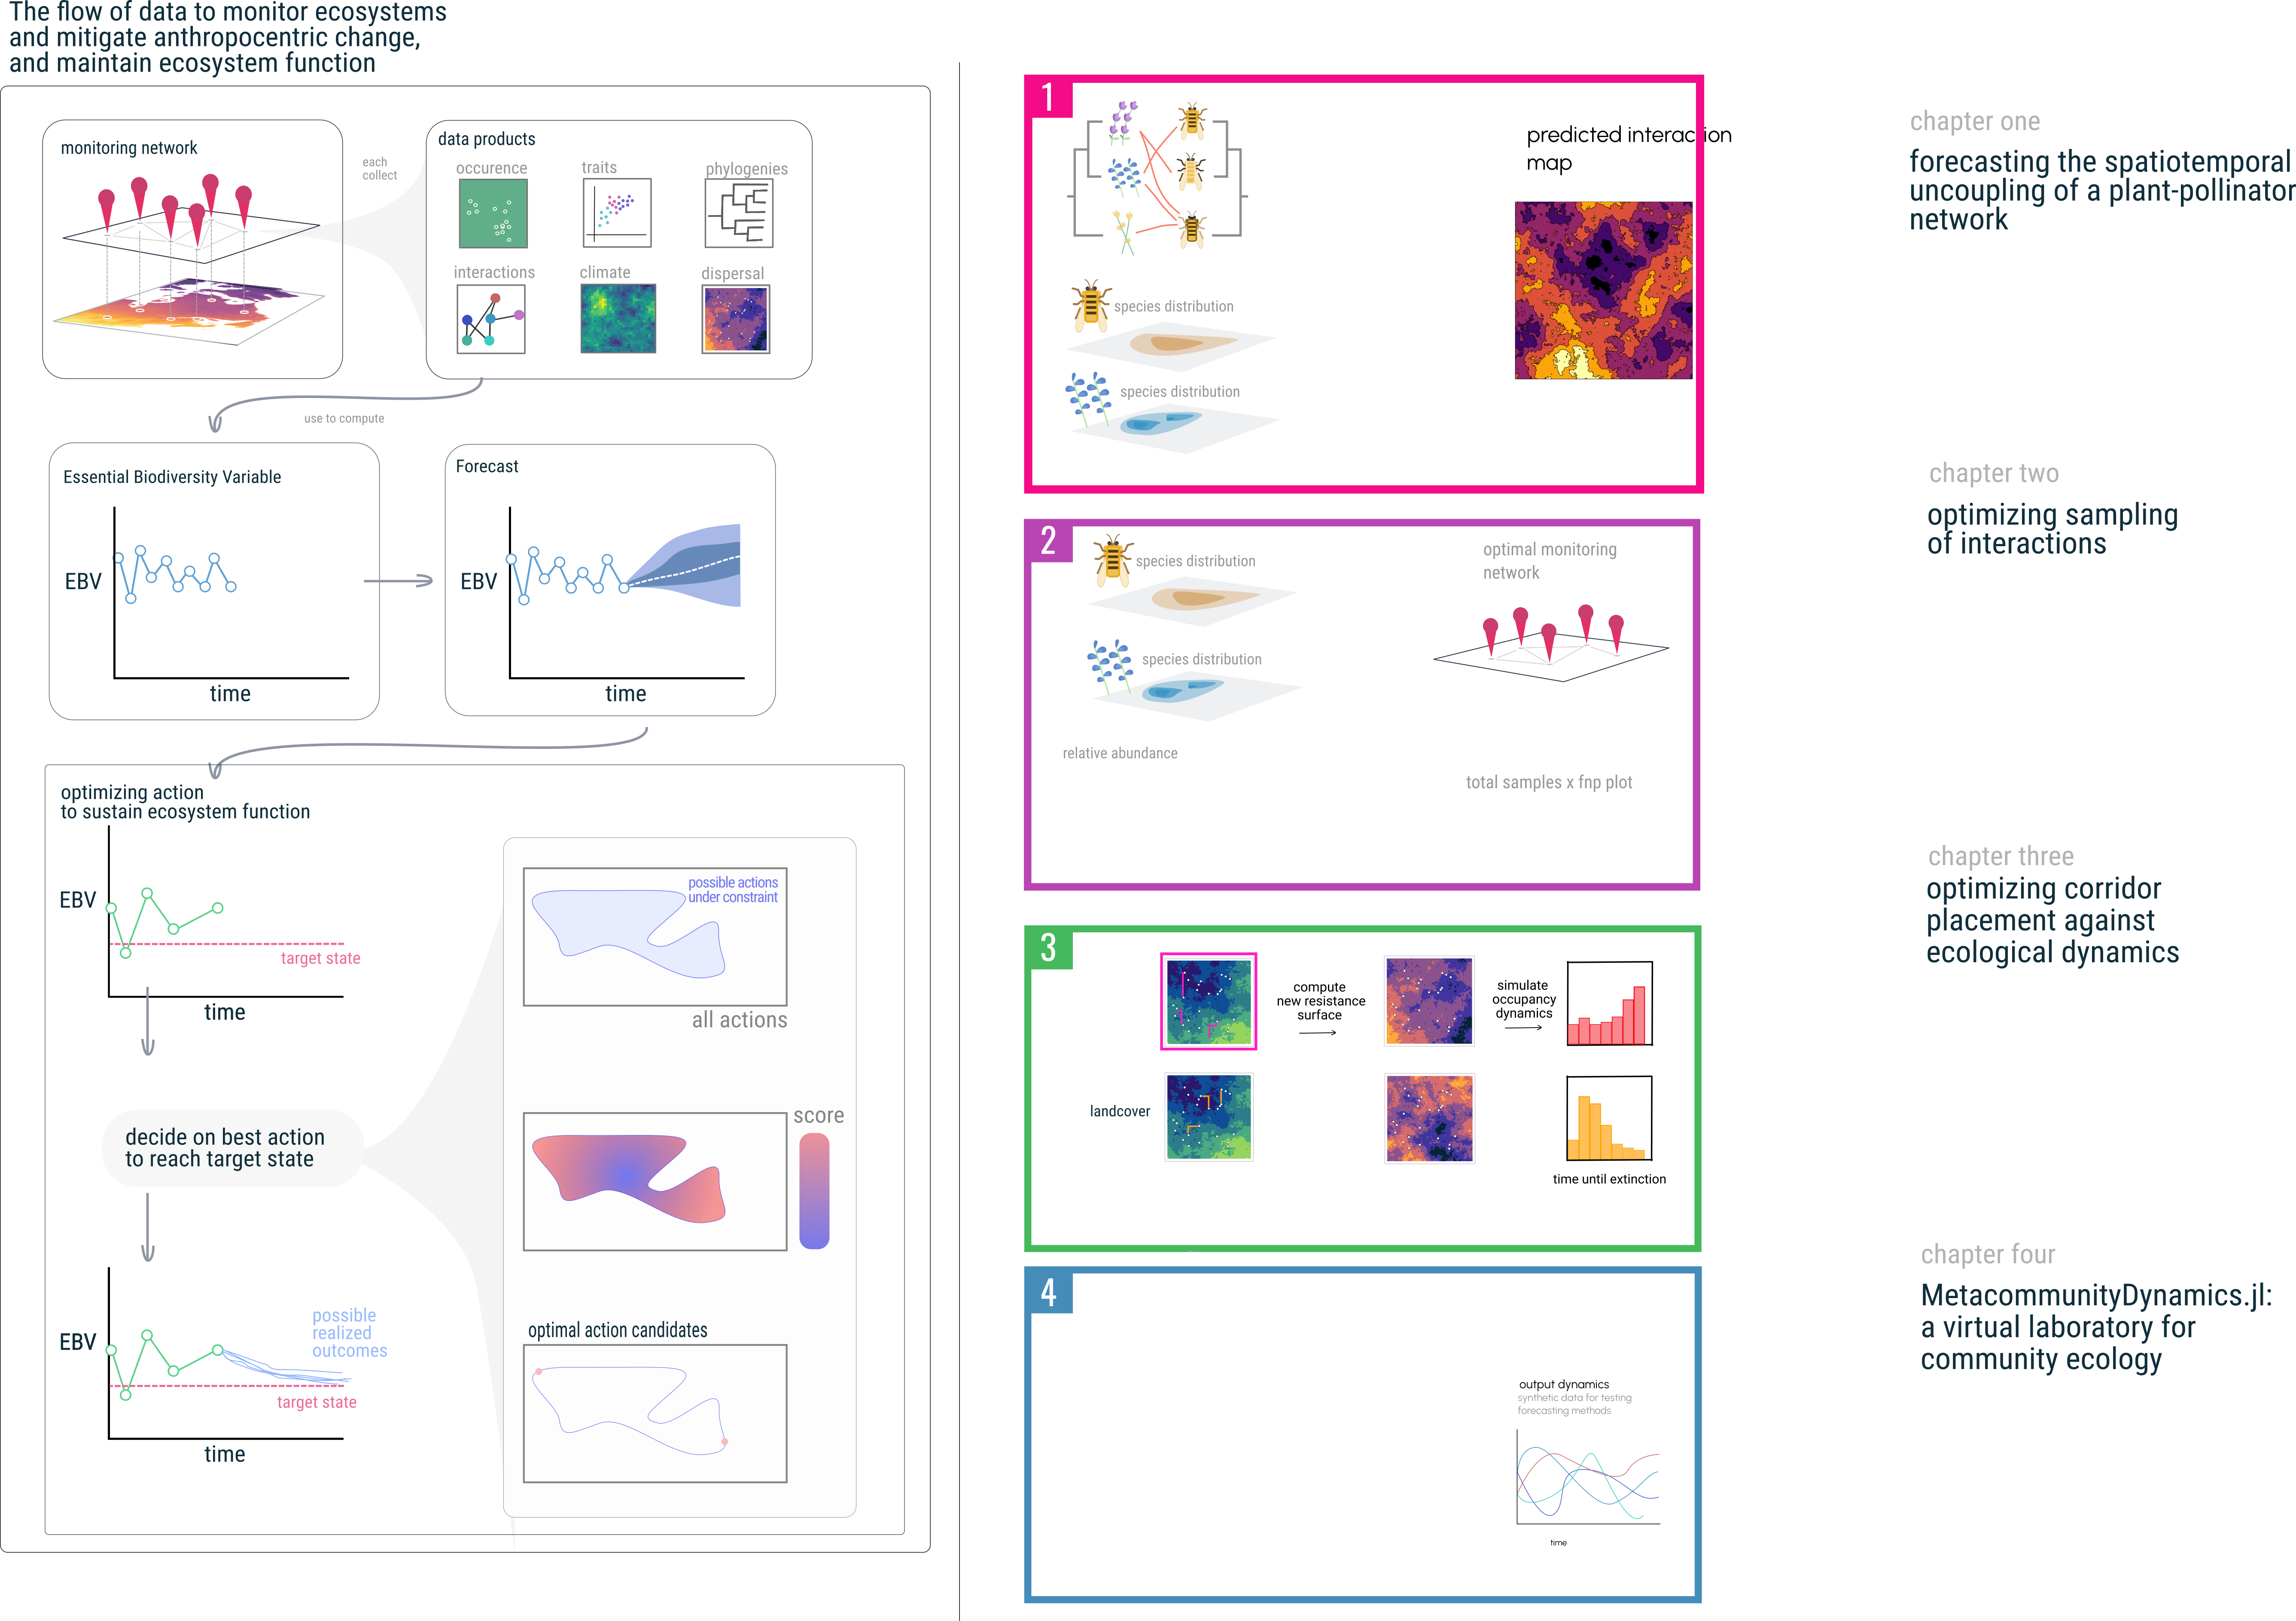
\includegraphics{./figures/thesisconcept.png}
\caption{thesis concept}
\end{figure}

\hypertarget{ch1-optimizing-sampling-of-species-distributions}{%
\section{CH1 optimizing sampling of species
distributions}\label{ch1-optimizing-sampling-of-species-distributions}}

\begin{itemize}
\tightlist
\item
  simulate species distribution and efficacy of detection given a set of
  observation points where the dist from observation site decays.
\item
  optimize set of repeated sampling locations L for a \emph{known}
  distribution D.
\item
  address SDM not being the territory
\end{itemize}

\hypertarget{ch2-optimizing-sampling-of-interactions}{%
\section{CH2 optimizing sampling of
interactions}\label{ch2-optimizing-sampling-of-interactions}}

\begin{itemize}
\tightlist
\item
  the missing link paper, turn this into optimizing with two different
  SDMs
\end{itemize}

\hypertarget{ch3-optimizing-corridor-placement}{%
\section{CH3 optimizing corridor
placement}\label{ch3-optimizing-corridor-placement}}

\begin{itemize}
\tightlist
\item
  land cover -\textgreater{} resistance -\textgreater{} extinction time
\item
  simulated annealing to optimize landscape optimization
\end{itemize}

\hypertarget{ch4-a-software-note-on-the-resulting-packages.}{%
\section{CH4 a software note on the resulting
packages.}\label{ch4-a-software-note-on-the-resulting-packages.}}

\begin{itemize}
\tightlist
\item
  \texttt{Observatories.jl}, \texttt{Corridors.jl}, \texttt{MCD.jl}
\end{itemize}

\end{document}
